\documentclass[11pt,a4paper]{article}
\usepackage[utf8]{inputenc}
\usepackage[T1]{fontenc}
\usepackage[spanish,es-nodecimaldot]{babel}
\usepackage{amsmath,amssymb,bm,booktabs,graphicx,geometry}
\usepackage[colorlinks=true,allcolors=blue]{hyperref}
\geometry{margin=25mm}
\graphicspath{{results/pose_measurement_independent_20260916_145207_467/}{results/pose_measurement_common_rotation_20260916_145855_607/}{results/actuation_independent_20260916_145900_208/}}
\title{Sensibilidad a errores de reorientación\\\large Distinción entre incertidumbre de pose y perturbación de actuación}
\author{Proyecto Cambridge}
\date{16 de septiembre de 2026}
\begin{document}
\maketitle

\section{Qué error se simula}
Se parte del modelo generalizado $\mu_i=\beta s_i^\nu$, con $\nu=m_R>0$, $s_i=\mathbf n_i^{\mathsf T}\mathbf u$ y $\beta=Cf_T(\mathbf u)/d^2$. Los estimadores LS, GLS, WLS y NLS ya implementados se reutilizan sin entregarles las orientaciones verdaderas cuando éstas son inciertas.

Los experimentos separan tres escenarios:
\begin{enumerate}
\item \textbf{Medición de pose, errores independientes}: las normales verdaderas se mantienen en el valor nominal del experimento. El algoritmo recibe normales estimadas con error angular. La cota elimina las poses verdaderas como parámetros auxiliares de una verosimilitud conjunta RSS--pose.
\item \textbf{Medición de pose, rotación común}: un mismo error de referencia de actitud afecta a todas las normales de un barrido. Se conserva su correlación, no se modelan sus efectos como ruidos independientes. El error se vuelve a generar entre ensayos: no es un sesgo determinista fijo durante toda la campaña.
\item \textbf{Actuación no observada}: las normales reales fluctúan respecto a los comandos, pero el algoritmo sólo recibe los comandos. La cota dibujada es una aproximación Gaussiana de momentos para pequeñas perturbaciones, no la CRLB exacta de una mezcla no lineal marginalizada.
\end{enumerate}
En todos los casos el error de una orientación se mantiene durante sus $N_i$ muestras ópticas; no se divide su varianza por $N_i$. La posición del centro óptico permanece constante. Los tilts de $3^\circ$ y $10^\circ$ indican puntos de operación nominales, no un recorte de la perturbación por topes mecánicos. Si existen topes, debe modelarse la distribución truncada correspondiente.

\section{Unidades y perturbaciones sobre la esfera}
Sea $E_i\in\mathbb R^{3\times2}$ una base ortonormal tangente a $\mathbf n_i$, con $E_i^{\mathsf T}\mathbf n_i=0$. Para errores independientes se usa:
\begin{equation}
 \boldsymbol\delta_i\sim\mathcal N(0,v_\theta I_2),\qquad
 \mathbf n_i(\boldsymbol\delta_i)=\cos\|\boldsymbol\delta_i\|\,\mathbf n_i+
 \frac{\sin\|\boldsymbol\delta_i\|}{\|\boldsymbol\delta_i\|}E_i\boldsymbol\delta_i.
\label{eq:perturb}
\end{equation}
La normal permanece unitaria. En cero se utiliza el límite del cociente. Para error común se utiliza una rotación de Rodrigues de vector $\boldsymbol\omega\sim\mathcal N(0,v_\theta I_3)$ aplicada a todas las normales.

El eje horizontal de las gráficas es la \emph{varianza por componente angular en grados cuadrados}. La conversión es:
\begin{equation}
 v_\theta=v_{\rm deg^2}\left(\frac\pi{180}\right)^2,\qquad
 \sigma_{\rm deg}=\sqrt{v_{\rm deg^2}}.
\end{equation}
Para perturbaciones pequeñas, el RMS del ángulo total de una normal es aproximadamente $\sqrt2\,\sigma_{\rm deg}$ en ambos modelos isotrópicos. No se está asignando esa misma varianza al azimut bruto del gimbal. En coordenadas inclinación--azimut, una perturbación pequeña satisface:
\begin{equation}
 \Delta\mathbf n\simeq\mathbf t_\theta\Delta\theta+
 \sin\theta\,\mathbf t_\alpha\Delta\alpha.
\end{equation}
Por ello una varianza de azimut tiene un efecto normal proporcional a $\sin^2\theta$. Antes de usar especificaciones de encoders debe transformarse su covarianza a las coordenadas de error elegidas.

\section{PEB con mediciones de pose inciertas}
Se modelan las poses verdaderas mediante coordenadas locales desconocidas $\boldsymbol\delta$, y observaciones auxiliares $\hat{\boldsymbol\delta}=\boldsymbol\delta+\mathbf e$, con covarianza conocida $V_\theta$. El punto verdadero de la comparación es $\boldsymbol\delta=0$, pero no se entrega ese valor al estimador. El sensor entrega coordenadas ruidosas, que se convierten en normales mediante \eqref{eq:perturb}. Elegir un punto nominal verdadero no significa asumir que el error real es conocido.

Si $J=\partial\bm\mu/\partial\mathbf r^{\mathsf T}$ y $D=\partial\bm\mu/\partial\boldsymbol\delta^{\mathsf T}$, con $\Sigma=\operatorname{diag}(\sigma^2/N_i)$, la FIM conjunta es \cite{kay}:
\begin{equation}
 I_{r,\delta}=\begin{bmatrix}
 J^{\mathsf T}\Sigma^{-1}J & J^{\mathsf T}\Sigma^{-1}D\\
 D^{\mathsf T}\Sigma^{-1}J & D^{\mathsf T}\Sigma^{-1}D+V_\theta^{-1}
 \end{bmatrix}.
\end{equation}
Su complemento de Schur proporciona la información equivalente de posición:
\begin{align}
 I_e&=J^{\mathsf T}\Sigma^{-1}J-J^{\mathsf T}\Sigma^{-1}D
 (D^{\mathsf T}\Sigma^{-1}D+V_\theta^{-1})^{-1}D^{\mathsf T}\Sigma^{-1}J,\\
 &=J^{\mathsf T}(\Sigma+DV_\theta D^{\mathsf T})^{-1}J,\qquad
 \mathrm{PEB}_{\rm pose}=\sqrt{\operatorname{tr}(I_e^{-1})}.
\label{eq:posebound}
\end{align}
La igualdad se obtiene por la identidad de Woodbury. Para errores independientes, la fila $i$ de $D$ sólo tiene dos entradas no nulas:
\begin{equation}
 D_{i,\{2i-1,2i\}}=\beta\nu s_i^{\nu-1}\mathbf u^{\mathsf T}E_i.
\end{equation}
Con $V_\theta=v_\theta I$, el incremento diagonal de covarianza equivalente es:
\begin{equation}
 (DV_\theta D^{\mathsf T})_{ii}=v_\theta\beta^2\nu^2s_i^{2\nu-2}(1-s_i^2).
\end{equation}
Para una rotación común, las filas tienen tres componentes:
\begin{equation}
 D_{i,:}=\beta\nu s_i^{\nu-1}(\mathbf n_i\times\mathbf u)^{\mathsf T}.
\end{equation}
En ese caso $DV_\theta D^{\mathsf T}$ no es diagonal. Ignorar su correlación no representa el mismo problema de actitud global.

\textbf{Interpretación:} \eqref{eq:posebound} es una CRLB local del modelo conjunto con mediciones auxiliares de pose y ruido independiente conocido, en regiones regulares. No se añaden derivadas de la matriz equivalente como si ésta fuera la covarianza de una nueva observación marginal: aquí resulta de eliminar parámetros auxiliares de la verosimilitud original. Aumentar $v_\theta$ aumenta esa matriz equivalente en orden semidefinido, por lo que el PEB de pose no disminuye. En $v_\theta=0$ se recupera el PEB con orientaciones perfectamente conocidas.

Los cuatro algoritmos de comparación utilizan la pose estimada como si fuera exacta; no resuelven una optimización conjunta de las poses individuales y la posición. Por ello no tienen por qué alcanzar esta cota. El orden relativo entre algoritmos puede cambiar al introducir errores de modelo.

\section{Perturbación de actuación no observada}
Aquí se generan normales reales con \eqref{eq:perturb} y potencias con el canal no lineal completo. El estimador recibe las normales nominales. No existen observaciones auxiliares de pose equivalentes a las de la sección anterior, por lo que no se presenta su complemento de Schur como la CRLB exacta de actuación.

Para error independiente, una expansión de la media hasta segundo orden angular y de la varianza hasta primer orden en $v_\theta$ da:
\begin{align}
 \bar\mu_i&\simeq\beta\left[s_i^\nu+v_\theta\left(-\nu s_i^\nu+
 \frac{\nu(\nu-1)}2s_i^{\nu-2}(1-s_i^2)\right)\right],\\
 V_i&\simeq\frac{\sigma^2}{N_i}+v_\theta\beta^2\nu^2s_i^{2\nu-2}(1-s_i^2).
\label{eq:moments}
\end{align}
La aproximación Gaussiana de momentos tiene varianza dependiente de posición. Su FIM debe incluir ambas contribuciones:
\begin{equation}
 [I_{\rm mom}]_{ab}=\sum_i\left[
 \frac{\partial_a\bar\mu_i\partial_b\bar\mu_i}{V_i}
 +\frac{\partial_aV_i\partial_bV_i}{2V_i^2}\right].
\label{eq:momentfim}
\end{equation}
El código deriva tanto media como varianza y valida sus gradientes por diferencias centrales. La curva se identifica siempre como \emph{Gaussian moment PEB (approx.)}. No es una integración exacta sobre las orientaciones latentes. La aproximación pierde fidelidad para errores grandes, cerca de cambios de máscara FOV y cuando términos de orden superior dominan, por ejemplo cerca de alineación donde la primera derivada angular es pequeña. No se afirma monotonía universal de esta aproximación por el mismo argumento usado en \eqref{eq:posebound}.

El PEB nominal de orientaciones exactas se conserva como línea de referencia. Perturbar las normales y luego calcular un PEB suponiendo que el algoritmo conoce esas normales perturbadas sería un experimento con información de oráculo. Podría incluso mejorar la diversidad angular y no mediría el daño de desconocer la orientación; no es el procedimiento utilizado aquí.

\section{Configuración, métricas y resultados}
Los scripts usan por defecto $m_R=1$, $K=9$, $\Phi_{1/2}=45^\circ$, FOV $46^\circ$, $P_t=0.65$ W, área $75.4\ \mathrm{mm}^2$ y $N_i=1000$. Se comparan conos nominales de $3^\circ$ y $10^\circ$ en 18 posiciones con $x,y\in\{-0.3,0,0.3\}$ m y $z\in\{0.5,1.1\}$ m. Cada configuración utiliza 150 ensayos. Las varianzas ensayadas son $0,0.0025,0.01,0.04,0.16,0.49,1$ grados cuadrados por componente.

Se guardan observaciones RSS, perturbaciones y sus coordenadas, estimaciones, errores, estados y parámetros. Las mismas observaciones se usan para todos los métodos; se conservan semillas y se restaura el generador aleatorio al finalizar. Los fallos permanecen en las estadísticas y se muestra además la fracción de ensayos con desacuerdo entre máscaras de visibilidad verdadera y asumida. En las configuraciones ejecutadas esa fracción fue cero; esto no garantiza validez a varianzas mayores o en otros dominios.

Como referencia, el PEB nominal espacial es aproximadamente 1.959 cm para tilt $3^\circ$ y 0.591 cm para tilt $10^\circ$. En varianza $1\ \mathrm{deg}^2$ se obtiene:
\begin{center}
\begin{tabular}{llrr}
\toprule
Modelo & Tilt & PEB [cm] & RMSE NLS [cm] \\
\midrule
Pose independiente & $3^\circ$ & 8.114 & 8.392 \\
Pose independiente & $10^\circ$ & 2.671 & 3.184 \\
Actitud común & $3^\circ$ & 4.807 & 4.824 \\
Actitud común & $10^\circ$ & 4.430 & 4.409 \\
Actuación independiente & $3^\circ$ & 7.441 (aprox.) & 8.215 \\
Actuación independiente & $10^\circ$ & 2.636 (aprox.) & 3.142 \\
\bottomrule
\end{tabular}
\end{center}
Los valores Monte Carlo pueden quedar ligeramente por debajo de una cota local por incertidumbre de muestreo o sesgo; no se fuerza una desigualdad artificial en las curvas. LS y NLS siguen coincidiendo en estas simulaciones de $m_R=1$ porque resuelven el mismo ajuste de potencias con las normales entregadas, aunque éstas sean incorrectas.

El error independiente se amplifica fuertemente con poca diversidad angular. Un error común de actitud es otro mecanismo: no desaparece simplemente aumentando muestras RSS, y cambiar el cono no elimina la incertidumbre de la referencia global. Más área o potencia tampoco elimina necesariamente el límite impuesto por pose: cuando domina $DV_\theta D^{\mathsf T}$, éste y la información de señal escalan conjuntamente con la ganancia óptica.

\begin{figure}[htbp]\centering
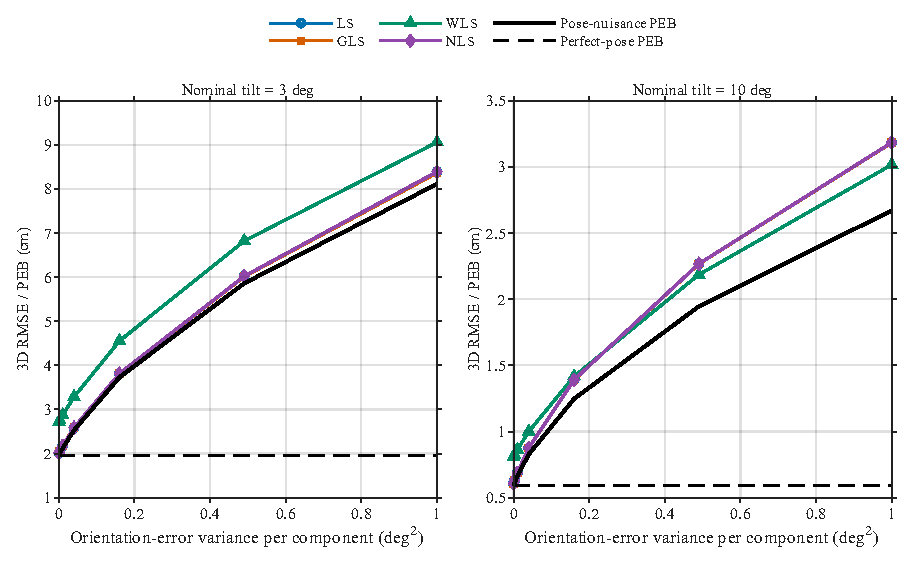
\includegraphics[width=0.96\linewidth]{Orientation_sensitivity_pose_measurement_independent.pdf}
\caption{Normales verdaderas fijas y medidas de pose independientes con incertidumbre. La curva negra continua es el PEB con poses auxiliares; la discontinua supone pose perfecta.}
\end{figure}
\begin{figure}[htbp]\centering
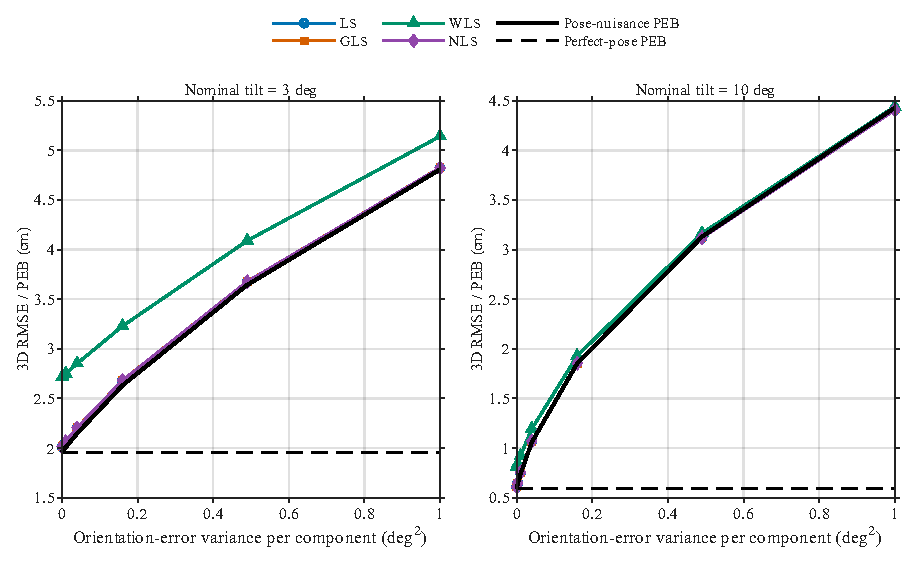
\includegraphics[width=0.96\linewidth]{Orientation_sensitivity_pose_measurement_common_rotation.pdf}
\caption{Error común de actitud, correlacionado a través de las orientaciones del barrido. No se sustituye la covarianza común por una diagonal.}
\end{figure}
\begin{figure}[htbp]\centering
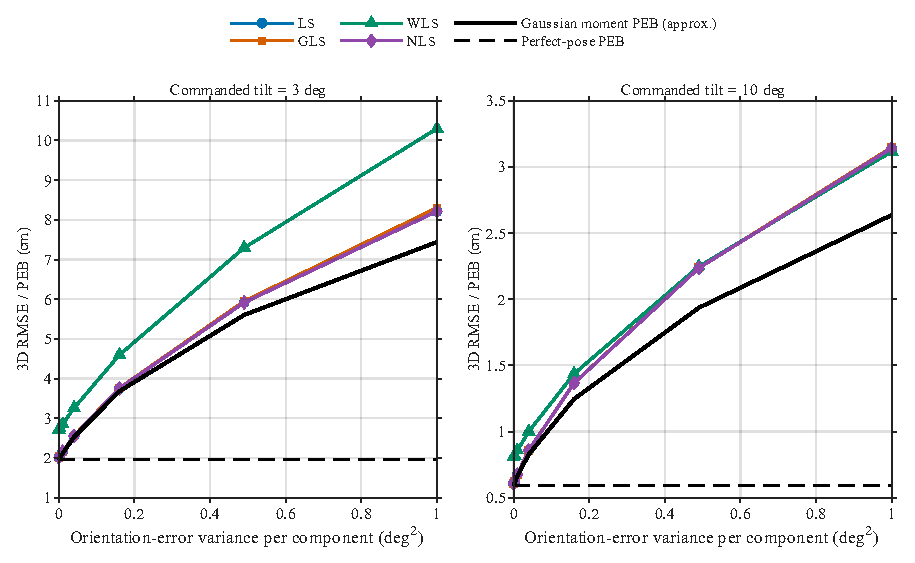
\includegraphics[width=0.96\linewidth]{Orientation_sensitivity_actuation_independent.pdf}
\caption{Actuación perturbada no observada por el algoritmo. La referencia de momentos es aproximada y se distingue de la CRLB del modelo con mediciones de pose.}
\end{figure}

\section{Uso e interpretación práctica}
\begin{itemize}
\item \path{sim01_pose_measurement_error.m}: errores independientes de conocimiento de las normales.
\item \path{sim02_actuation_error.m}: errores de actuación no medidos, con referencia Gaussiana aproximada.
\item \path{sim03_common_attitude_error.m}: error correlacionado de referencia global.
\end{itemize}
Los campos \texttt{orientation\_variances\_deg2}, \texttt{cases}, \texttt{trials}, \texttt{mode} y \texttt{structure} son editables al principio. Los cálculos de cotas están separados en \texttt{rx\_pose\_error\_peb} y \texttt{rx\_actuation\_peb}; los algoritmos se reutilizan desde \path{Estimators}. El caso de varianza cero se comprobó contra la misma realización de Monte Carlo nominal; también se verificaron el complemento de Schur, las derivadas de momentos y la conservación de normales unitarias.

Para un sistema real se debe medir qué errores son independientes por orientación, cuáles son sesgos comunes y cuáles varían durante la adquisición. No se identifica una tolerancia de hardware universal a partir de estas curvas: depende de geometría, patrón, SNR, calibración y modelo estadístico. Una matriz de covarianza de encoders o IMU debe convertirse a la parametrización utilizada. Las simulaciones no incluyen traslación del pivote, deriva de ganancia ni movimiento del receptor.

\bibliographystyle{IEEEtran}
\bibliography{../Estimators/estimator_references}
\end{document}
